\section{Icke sinusformade signaler}
\textbf{HAREC a.\ref{HAREC.a.1.7}\label{myHAREC.a.1.7}}

\subsection{Grundton, övertoner- Kantvågor}
\textbf{HAREC a.\ref{HAREC.a.1.7.2}, a.\ref{HAREC.a.1.7.3}, a.\ref{HAREC.a.1.7.4b}\label{myHAREC.a.1.7.2}\label{myHAREC.a.1.7.3}\label{myHAREC.a.1.7.4b}}
\index{grundton}
\index{överton}
\index{kantvåg}

\begin{figure*}
\begin{center}
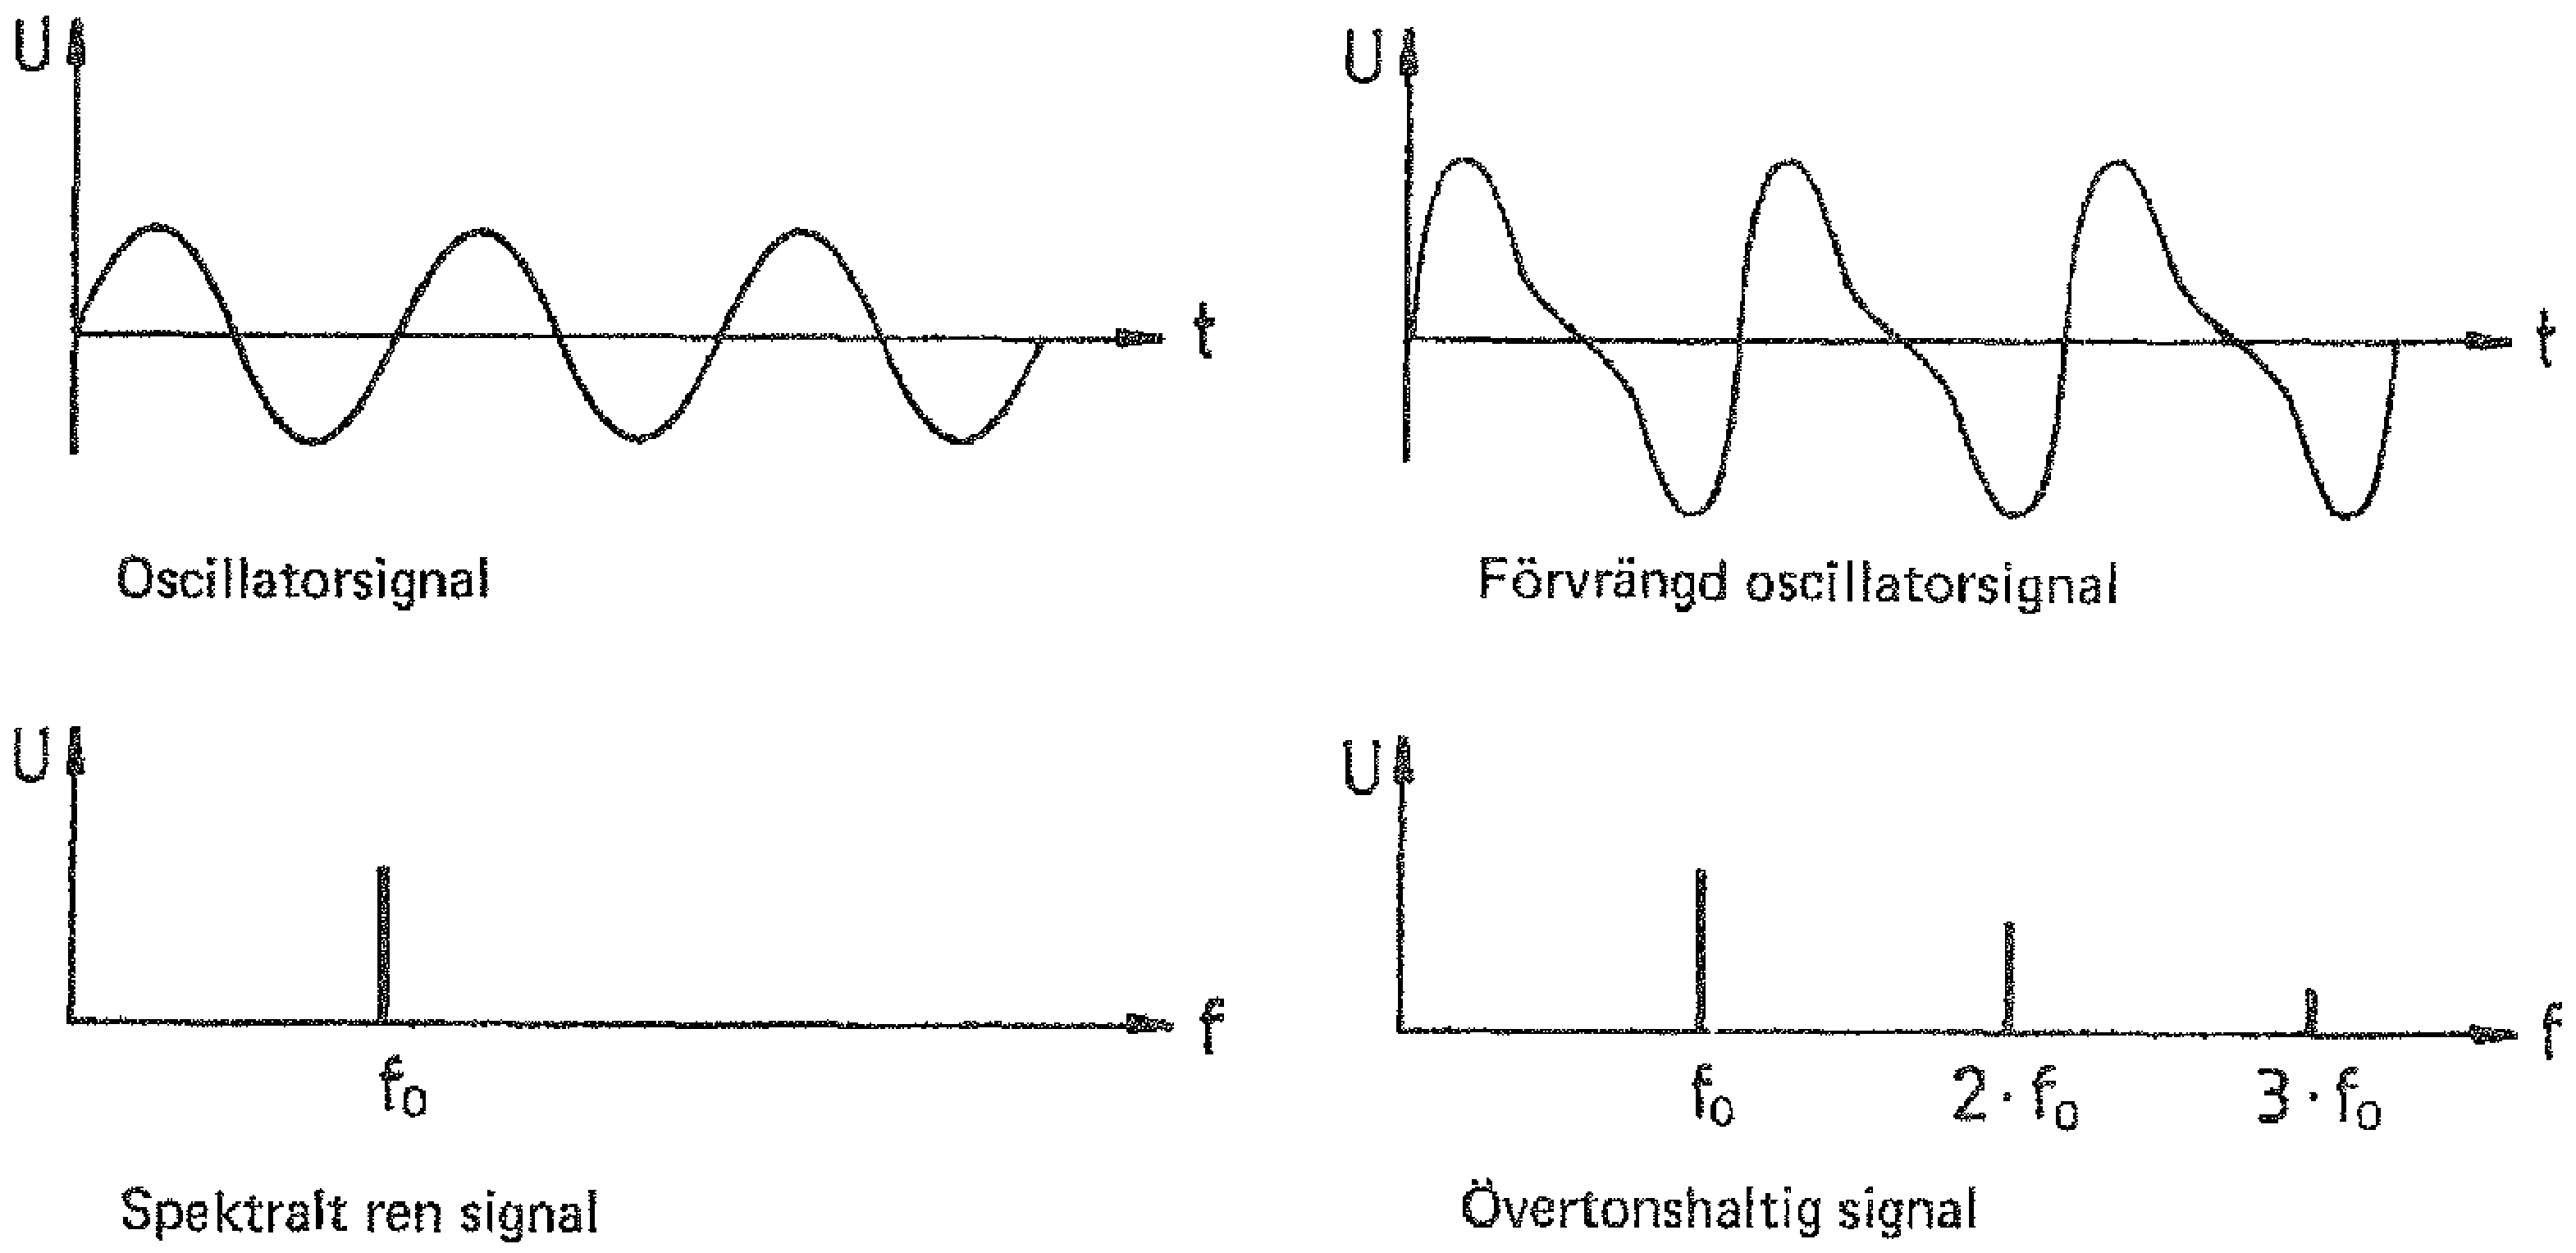
\includegraphics[width=\textwidth]{images/cropped_pdfs/bild_2_1-18.pdf}
\caption{Ren sinusvåg och övertonshaltig våg}
\label{fig:BildII1-18}
\end{center}
\end{figure*}

Bild \ref{fig:BildII1-18} visar en ren sinusvåg och övertonshaltig våg.
Ett sinusformat förlopp med en enda frekvens -- en enda ton -- sägs vara
spektralt ren.
En sådan svängning kallas för grundton.

Varje signal, som inte är sinusformad, är sammansatt av flera sinussvängningar.
Det är signalens grundton samt dess harmoniska övertoner, vilka kan ha 2, 3
o.s.v. gånger högre frekvens än grundtonen.
Den inbördes styrkan på grundton och övertoner avgör signalens form.
Om signalen ligger inom det hörbara området, kan man märka hur den ändrar
karaktär beroende på övertonshalten.
Man kan säga att övertonerna modulerar grundtonen.

\begin{figure*}
\begin{center}
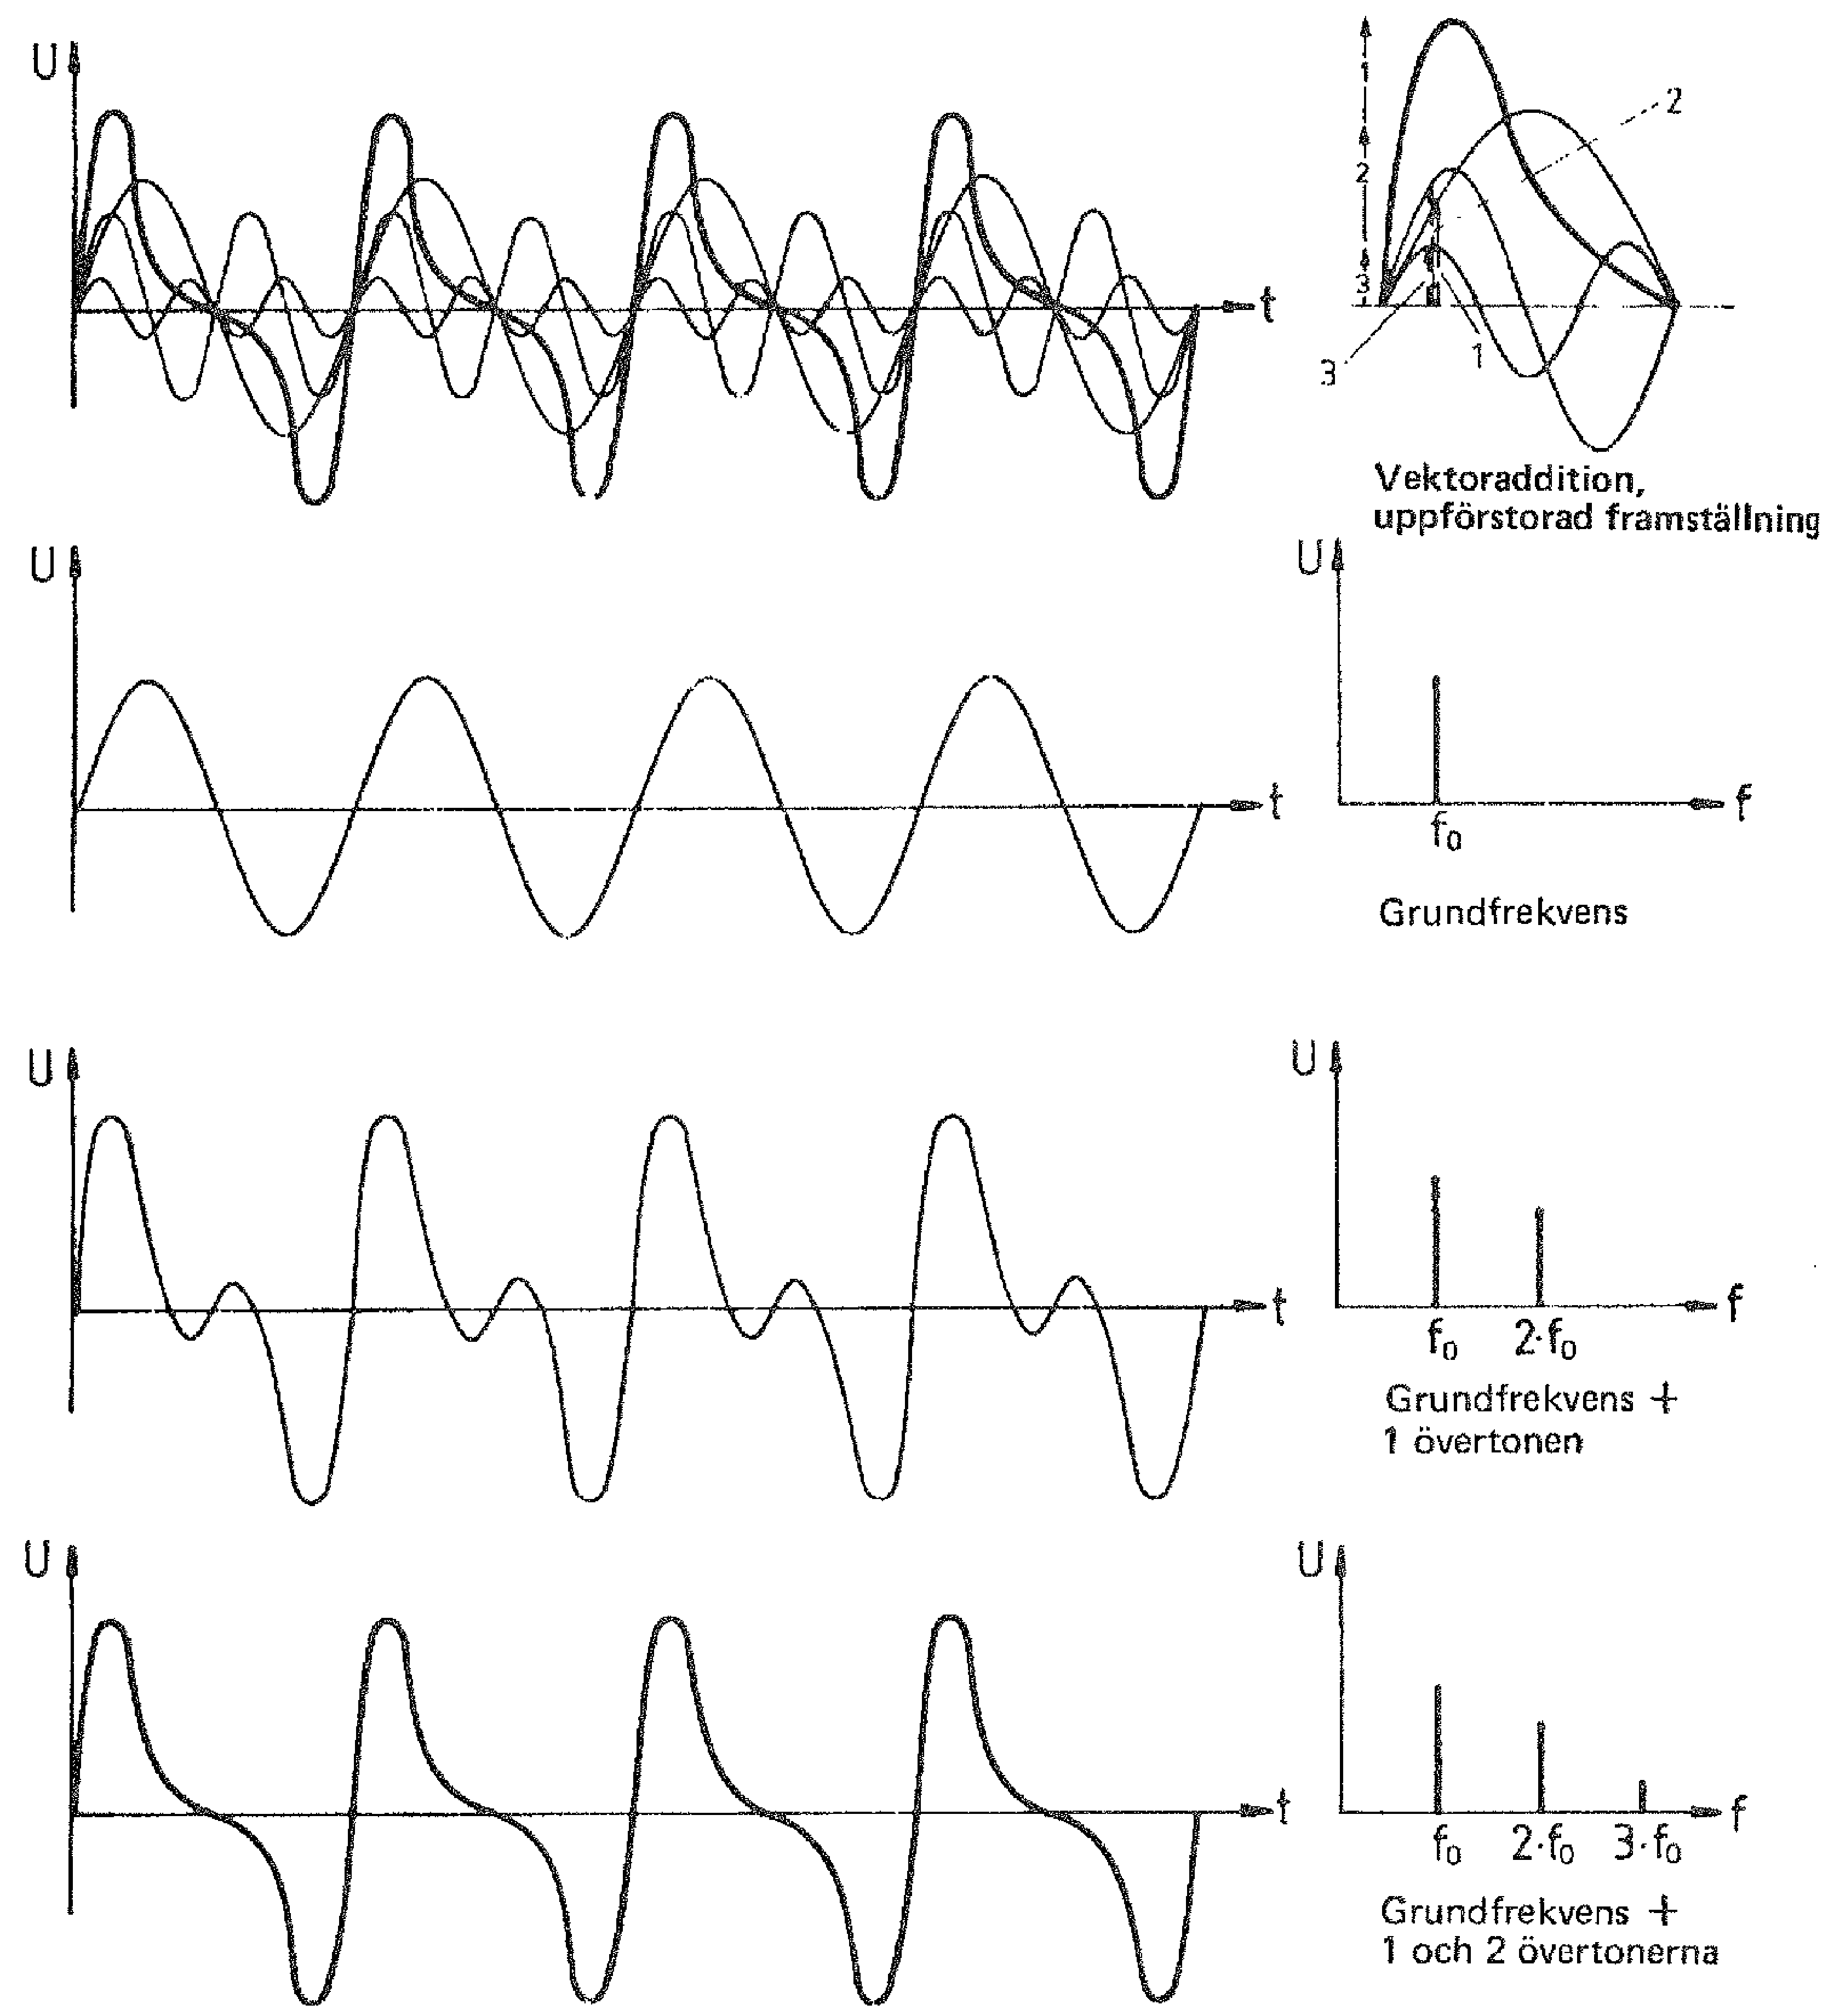
\includegraphics[width=\textwidth]{images/cropped_pdfs/bild_2_1-19.pdf}
\caption{Uppdelning av en signal i grundton och övertoner}
\label{fig:BildII1-19}
\end{center}
\end{figure*}

Bild \ref{fig:BildII1-19} visar uppdelning av en signal i grundton och
övertoner.
Oscillatorsignalen i exemplet på bilden har 1 volts amplitud på grundtonen
\(f_0\) (1:a harmoniska), 0,7~volts amplitud på de 1:a övertonen
(2:a harmoniska) och 0,2~volts amplitud på den 2:a övertonen (3:e harmoniska).
Den totala amplituden blir emellertid inte summan av 1, 0,7 och 0,2~volt
eftersom de olika delspänningarnas toppvärden inte uppträder samtidigt.
I stället måste delspänningarna adderas vid varje tidpunkt för sig.

\begin{figure*}
\begin{center}
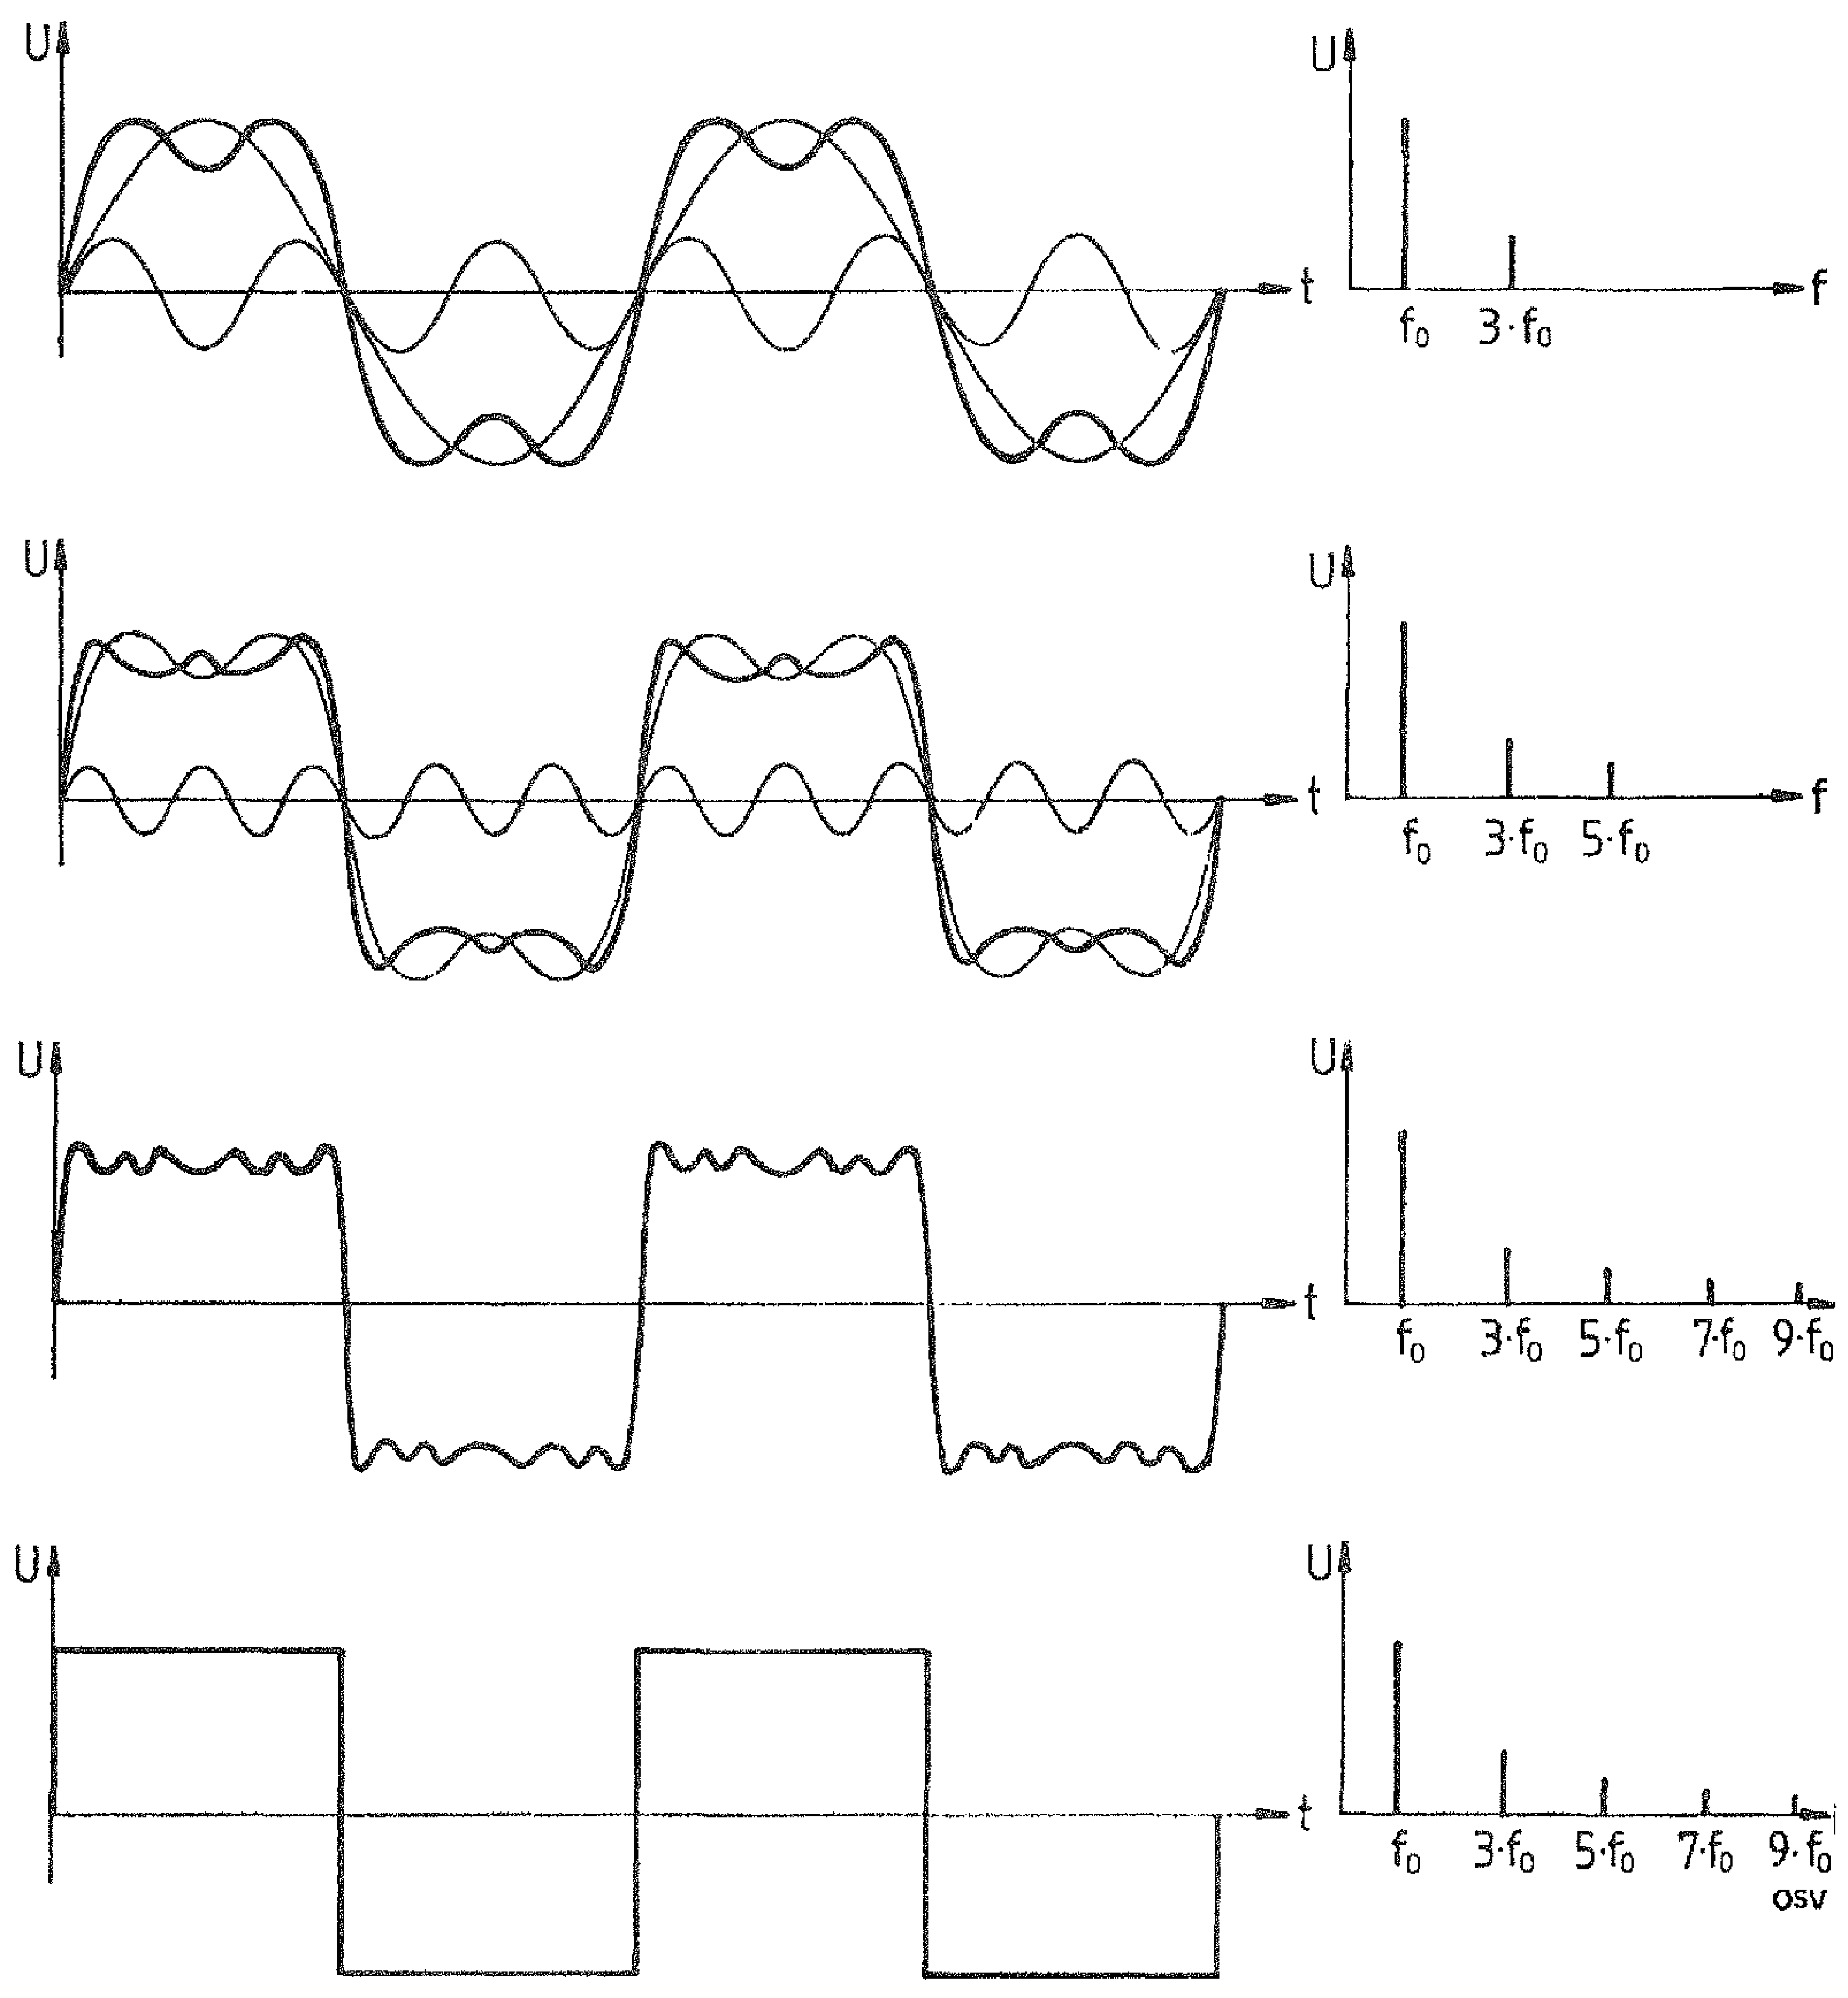
\includegraphics[width=\textwidth]{images/cropped_pdfs/bild_2_1-20.pdf}
\caption{Uppdelning av en fyrkantsvåg i grundton och övertoner}
\label{fig:BildII1-20}
\end{center}
\end{figure*}

Bild \ref{fig:BildII1-20} visar uppdelning av en fyrkantsvåg i grundton och
övertoner.

\index{Fourier, Joseph}
\index{Fourier!Fourier analys}
\index{Fourier!Fourier transform (FT)}
\index{Fourier!invers Fourier transform (IFT)}
\index{Fourier!Discrete Fourier Transform(DFT)}
\index{DFT}
\index{Fourier!inverse Discrete Fourier Transform (IDFT)}
\index{IDFT}
\index{Fourier!Fast Fourier Transform(FFT)}
\index{FFT}
\index{Fourier!inverse Fast Fourier Transform (IFFT)}
\index{IFFT}

\infobox{
Denna analys av vågor uppfanns av Jean-Baptiste Joseph Fourier (1768--1830)
vid analys av värmeutbredning och vibration som presenterades 1822.
Denna metod är kraftfull och har haft stort inflytande på vetenskapen och
utvecklingen både som matematiskt verktyg och som praktiskt analys med
spektrum-analysatorer och vid modern modulation och demodulation.
Man pratar om \emph{Fourier analys} (eng. Fourier analysis) och
\emph{Fourier transform (FT)} för omvandling från tid till frekvens och
\emph{invers Fourier transform} för omvandling från frekvens till tid.
För tidsdiskret (samplad) form är termerna
\emph{Diskret Fourier Transform (DFT)} och
\emph{invers Diskret Fourier Transform (IDFT)} respektive.
Senare optimeringar av beräkningar har resulterat i
\emph{Fast Fourier Transform (FFT)} och
\emph{Inverse Fast Fourier Transform (IFFT)}.
}

Det finns olika karaktärer av förlopp såsom sinusvåg, triangelvåg, sågtandsvåg,
fyrkantsvåg o.s.v.

Fyrkantsvågen är sammansatt av sinusvågor med grundfrekvensen och dess udda
övertoner, varvid amplituderna fördelar sig som \(1/1\), \(1/3\), \(1/5\),
\(1/7\), \(1/9\), \(1/11\) o.s.v.
Teoretiskt når övertonsspektrum upp till oändligt höga frekvenser, medan de
motsvarande amplituderna minskar till oändligt små värden.

En ideal fyrkantsvåg, vilken inte kan uppnås i praktiken, skulle bestå av ett
oändligt antal udda övertoner med fallande amplitud.
Ju fler av de högre övertonerna som filtreras bort, desto mer lutar
fyrkantsvågens flanker, desto rundare blir hörnen på vågen och desto vågigare
blir kurvans topp.

\subsection{Överlagrade spänningar
(likspänningskomposant)}
\textbf{HAREC a.\ref{HAREC.a.1.7.4a}\label{myHAREC.a.1.7.4a}}

\begin{figure}[ht]
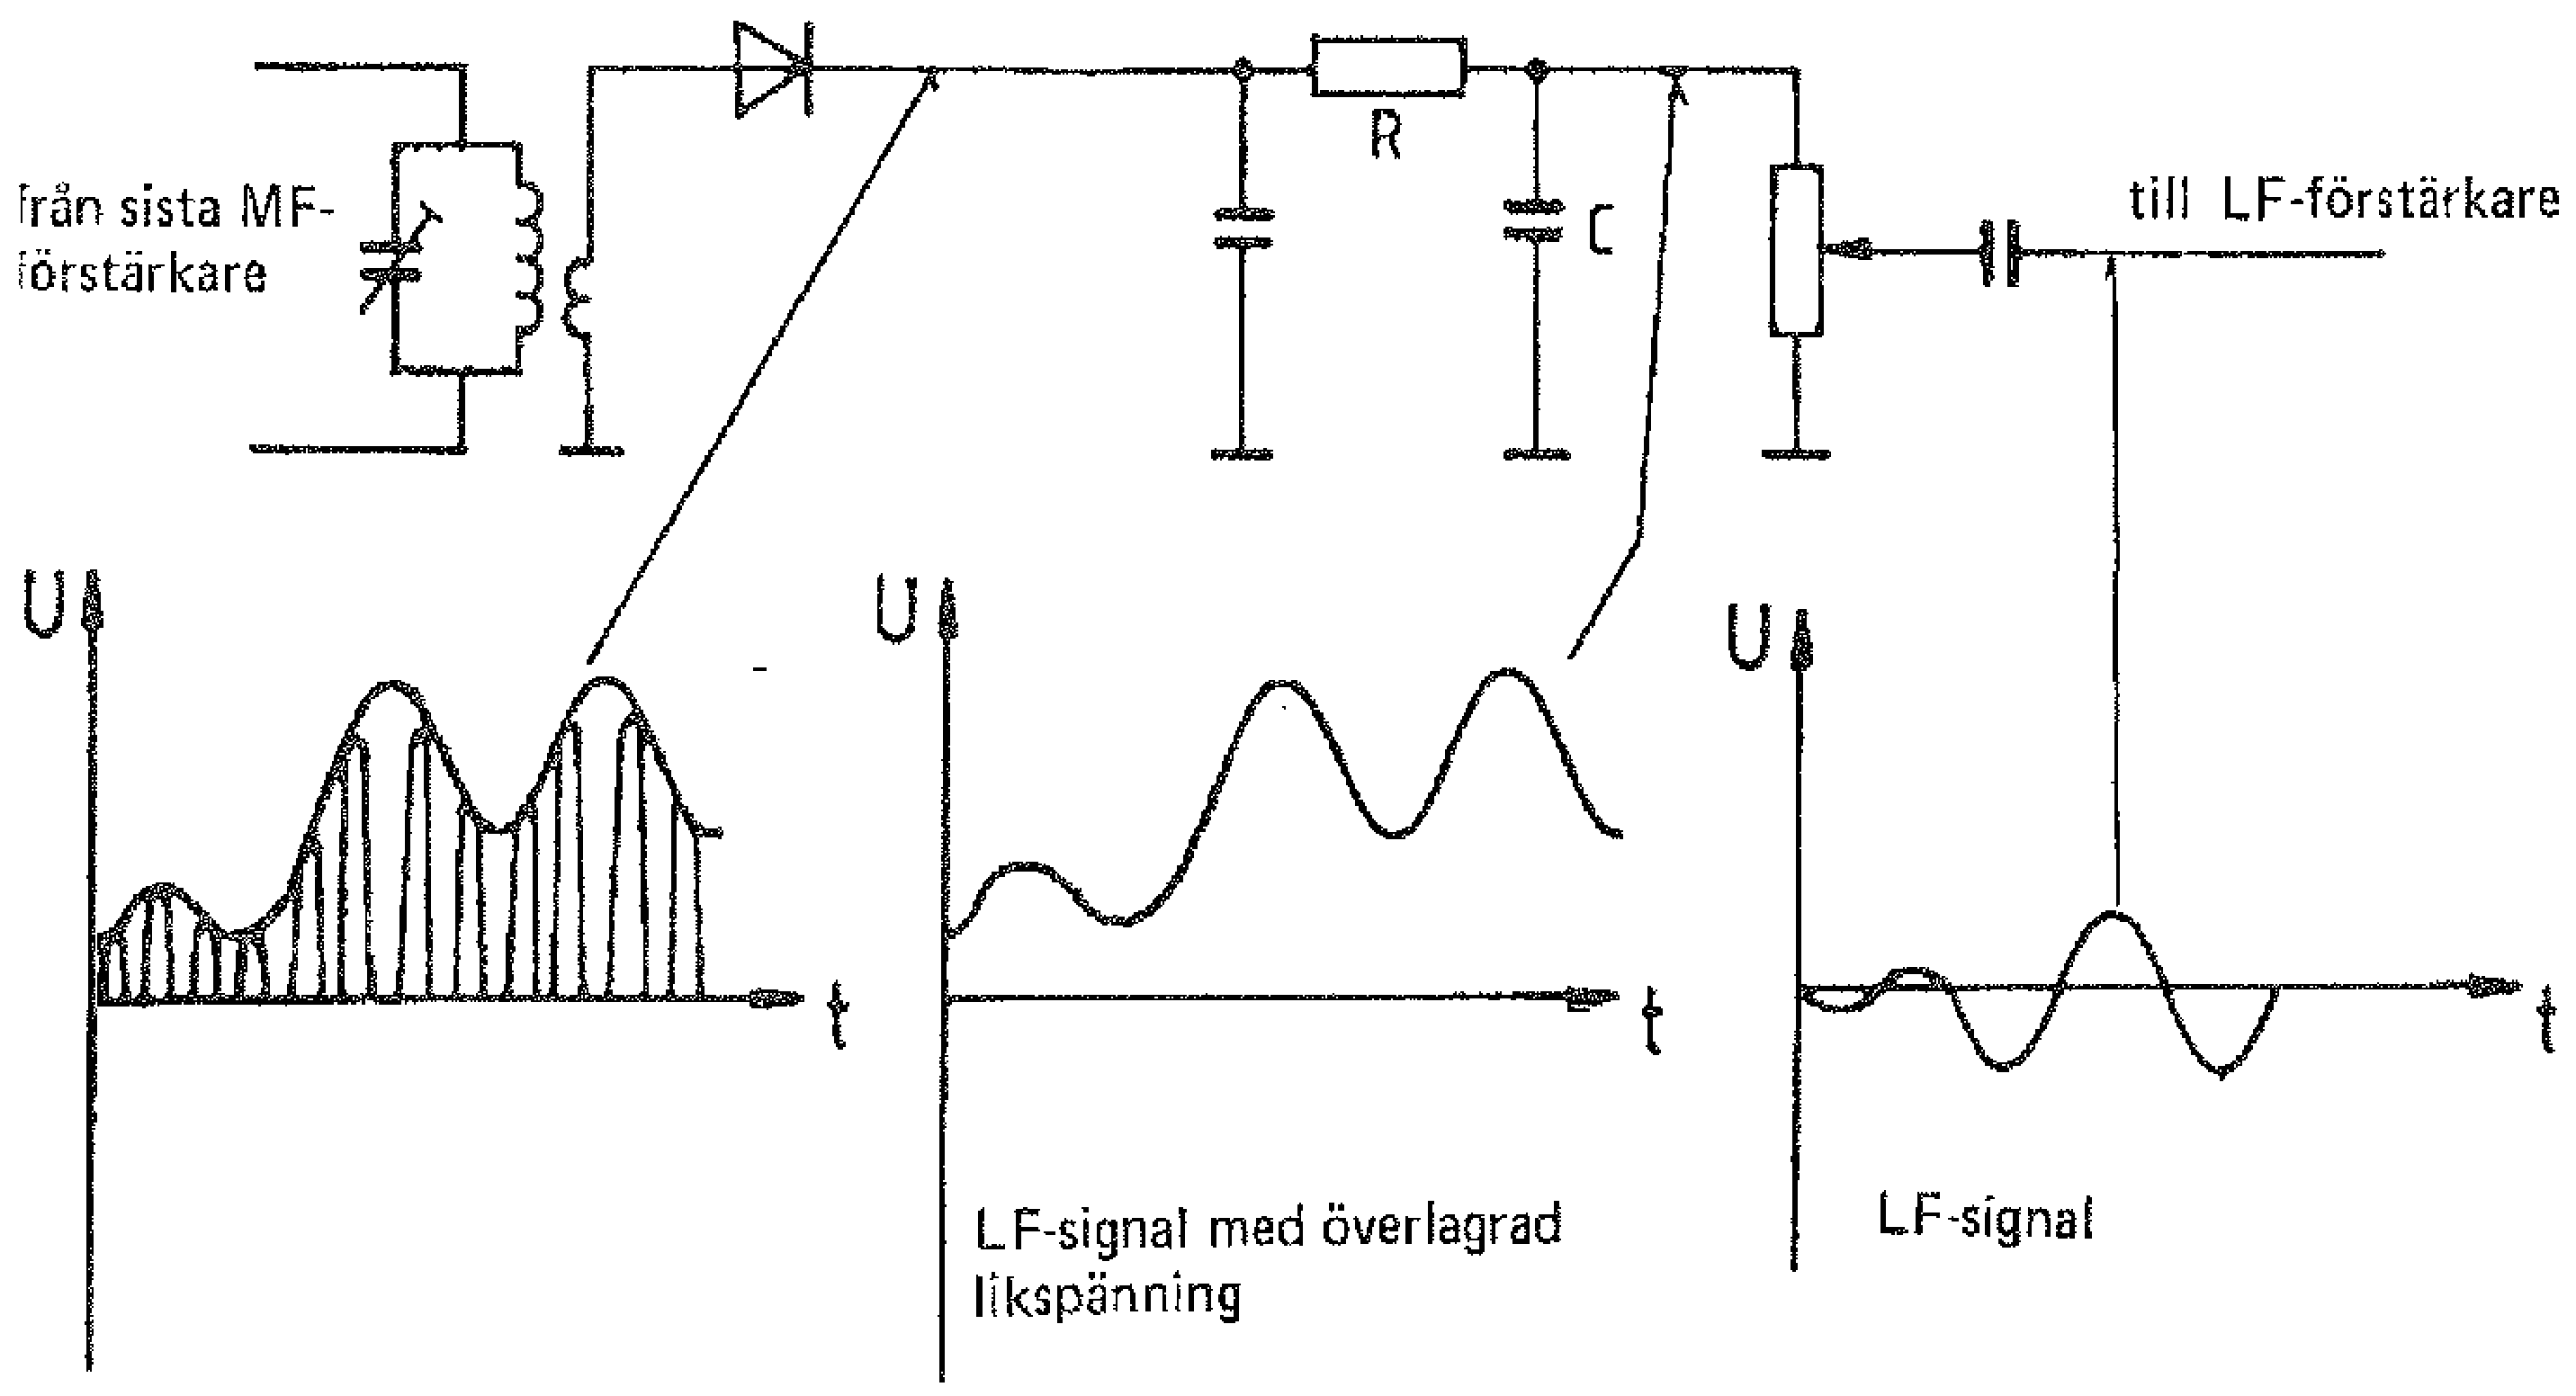
\includegraphics[width=\textwidth]{images/cropped_pdfs/bild_2_1-21.pdf}
\caption{Överlagrade spänningar}
\label{fig:BildII1-21}
\end{figure}

Bild \ref{fig:BildII1-21} visar överlagrade spänningar.
I signalkretsar förekommer det mycket ofta, att växelspänning överlagras på
likspänning eller omvänt.
Likspänningen kallas då för likspänningskomposant.
Olika åtgärder behövs för att överlagra spänningar på varandra och att sedan
skilja dem åt.

Bilden visar ett avsnitt av en AM-mottagare.
Från vänster hämtas en AM-modulerad signal från MF-förstärkaren för att
demoduleras, d.v.s. för att återvinna den modulerande LF-signalen.
MF-signalen halvvågslikriktas.
Kvar blir den positiva delen av MF-signalen och den modulerande LF-signalen,
sammanlagrade.
LF-signalen ska nu skiljas ut och förstärkas.
Alltså filtreras MF-komposanten bort.
Kvar blir LF-signalen, men överlagrad på en likspänning.
Likspänningen stoppas och kvar blir slutligen LF-signalen som förstärks.

\subsection{Brus}
\textbf{HAREC a.\ref{HAREC.a.1.7.5}\label{myHAREC.a.1.7.5}, a.\ref{HAREC.a.7.19}\label{myHAREC.a.7.19}}
\label{termisktbrus}

\subsubsection{Termiskt brus}
\index{brus}
\index{termiskt brus}
\index{brus!termiskt}

Resistorer och resistans, i alla dess former, uppvisar en egenskap av
en varierande spänning även när ingen ström går genom motståndet.
Denna extra spänning innehåller ett brett spektra av toner, men är också ett
tätt spektra, sådan att ingen enskild ton kan särskiljas från någon annan.
Istället för att tänka sig en grundton och dess övertoner med ingen energi
emellan dem så är det istället ett kontinuerligt spektra med oändligt många
toner.
Detta spektra begränsas dock av bandbredden.

\begin{wrapfigure}{R}{0.5\textwidth}
  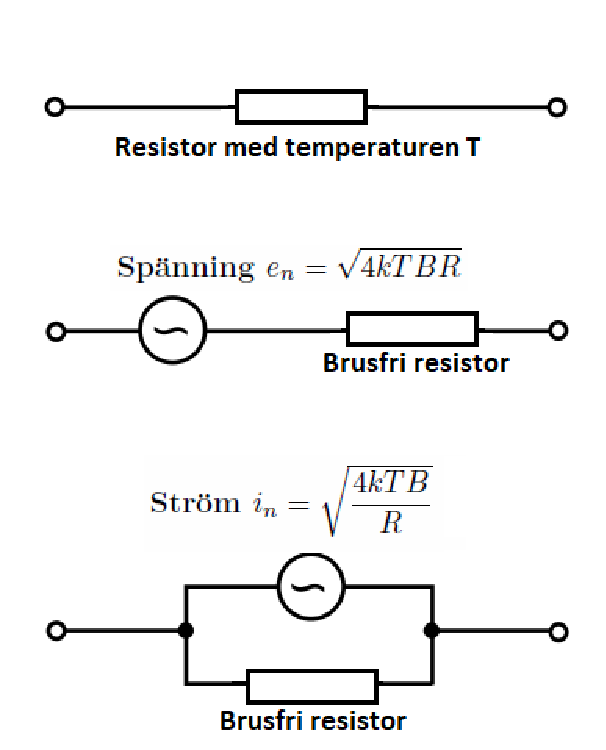
\includegraphics[width=0.5\textwidth]{images/cropped_pdfs/bild_2_1-36.pdf}
  \caption{En resistor kan ses ha brus ekvivalenter som spänning eller ström}
  \label{fig:BildII1-36}
\end{wrapfigure}

\begin{wrapfigure}{R}{0.5\textwidth}
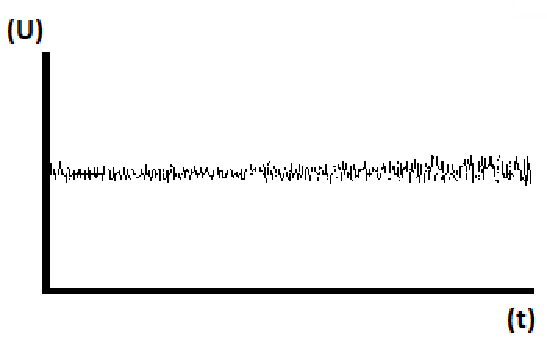
\includegraphics[width=0.5\textwidth]{images/cropped_pdfs/bild_2_1-34.pdf}
\caption{Brus innebär en ostabilitet över tid}
\label{fig:BildII1-34}
\end{wrapfigure}

\begin{wrapfigure}{R}{0.5\textwidth}
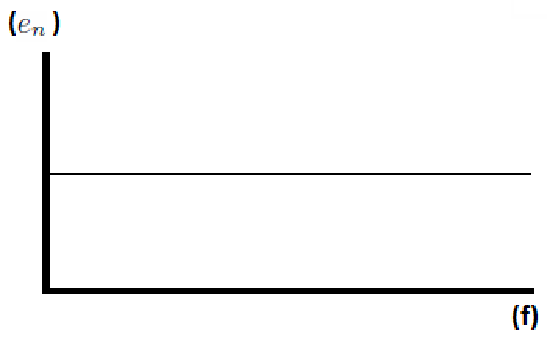
\includegraphics[width=0.5\textwidth]{images/cropped_pdfs/bild_2_1-35.pdf}
\caption{Brus innehåller alla frekvenser, vitt brus har samma amplitud}
\label{fig:BildII1-35}
\end{wrapfigure}

\index{vitt brus}
\index{brus!vitt}
\index{white noise}
\index{Johnsson noise}
\index{brus!Johnsson}
Man kallar detta spektra i daglig tal för \emph{termiskt brus}
(eng. thermal noise), eftersom det beror på temperaturen hos motståndet, eller
\emph{Johnsson noise}, efter J. B. Johnsson som 1928 fann att detta brus fanns
i alla ledare \cite{ott1988}.
Brus skapar en variation i spänning och ström, som illustreras i bild
\ref{fig:BildII1-34}.

I dagligt tal pratar man dock bara om \emph{vitt brus} (eng. white noise) eller
\emph{brus}.
Med vitt brus menas brus som inte ''färgats'', och det betyder i det här
sammanhanget att det har samma amplitud för alla frekvenser, så som illustreras
i bild \ref{fig:BildII1-35}.
I praktiken är allt brus begränsat med bandbredden på kanalen, men man
betraktar det som vitt inom kanalen om det är jämn inom bandet.

Effekten \(P_n\) av detta brus beror på Boltzmanns konstant
\(k\ =\ 1,38 \cdot 10^{-23}\) J/K, den absoluta temperaturen \(T\) i
kelvin samt bandbredden \(B\) i Hertz och anges enligt formeln:

\(P_n = k T B\)

Varje motstånd med den absoluta temperaturen T kan modelleras som att ha en
ekvivalent spänning \(e_n\) och ström \(i_n\) för resistansen \(R\),
så som illustreras i bild \ref{fig:BildII1-36} är

\(e_n = \sqrt{4kTBR}\)

\(i_n = \sqrt{\dfrac{4kTB}{R}}\)

\subsubsection{Brusbandbredd}
\index{brus!brusbandbredd}

Medans vi initialt antagit att brusets bandbredd är för frekvenser
från DC till övre gränsfrekvensen så är det inte nödvändigt.
Formeln är även relevant för bruset på ett band, och bandbredden för det
bandpass filter vi har för att enbart lyssna på detta band.

Exempelvis behöver tal på SSB hantera 300~Hz till 3~kHz, dvs. 2,7~kHz
bandbredd och därmed kommer även mottagarens bandbredd behöva vara så stort,
och därmed även brusbandbredd på 2,7~kHz.
Vi kommer då att ta emot brus för motsvarande bandbredd.
Ett CW filter kan t.ex. vara 350~Hz och kommer därmed också ha ett
motsvarande förhållande lägre brus-effekt.

Detta är dock en förenkling, eftersom filtret inte filtrerar med branta kanter
och är helt plant.
Filtrets egentliga brus-bandbredd beror på hur filtret filtrerar över
alla frekvenser och summan av dessa.
Beroende på vilken typ av filter så behövs därför en korrigeringsfaktor
från den normala bandbredden till brus-bandbredden.
För ett normalt 12~dB/oktav lågpass filter är korrigerings faktorn 1,22.
